\chapter{SLAM}\label{chp:slam_mapping}

One of the first challenges in indoor navigation for assistive robots is actually finding where they are. Robot localization is fundamental to not only know where the robot needs to go, but also find a path to avoid obstacles.

Mapping is an essential tool in this matter, and it connects the areas of \textit{concurrent mapping} and \textit{localization problem}. In themselves, both problems are relatively easy and well understood: mapping an environment knowing the localization and localizing the robot having the map in hands are simple tasks. However, the combination of those two problems is hard to solve \cite{thrun2000real}.

Many SLAM (Simultaneous Localization and
Map Building) algorithms emerged to try and solve these problems, using different approaches and a range of sensors to do the task. They also combine data from different sensors to provide higher precision. They often rely on assumptions about the system's nature. Some of the algorithms assume that the noise in the sensors can be modeled as a Gaussian distribution and that the movement of the robot is linear and apply Kalman Filters to predict the current state, based on the last state and the odometry data.

\section{Sensors}

The laser scanner (\figurename~\ref{fig:sick_s300_model}) is the most popular way to capture data about the environment. They work by sending beams of light in a direction and measuring the time it takes for the light to travel back and forth between the object and the sensor, either directly, by measuring time of flight, or indirectly, by measuring the phase-shift \cite{amann2001laser}. As you want the information to be gathered on more than a single point, the scanner can rotate a mirror or even the whole sensor to gather measurements from all directions, as shown on \prettyref{fig:sick_s300_diagram}. The LIDARs that do not contain moving parts are called solid state LIDARs.

\begin{figure}
     \centering
     \subfloat[][Sick S300 safety laser scanner.]{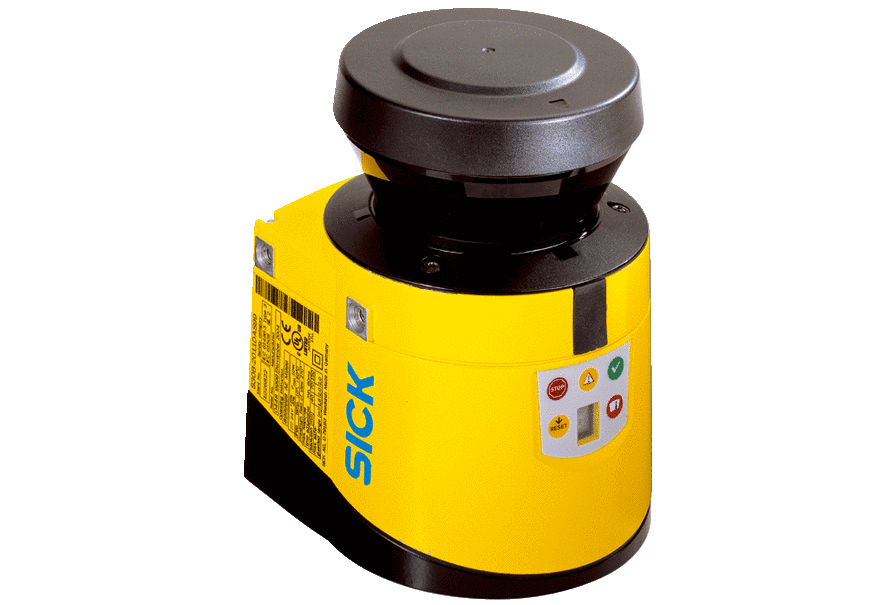
\includegraphics[width=80mm]{sick_s300}\label{fig:sick_s300_model}}
     \subfloat[][Sick S300 range diagram.]{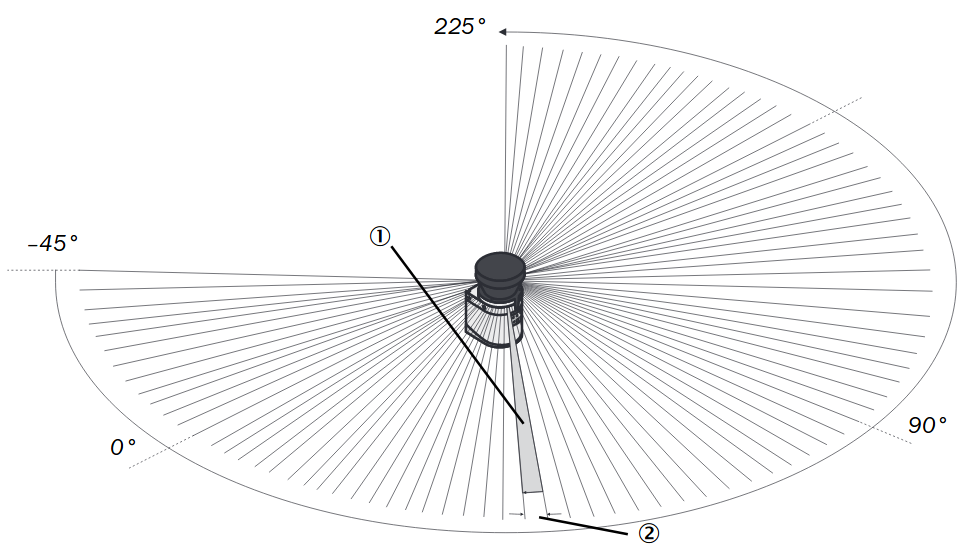
\includegraphics[width=80mm]{sick_s300_diagram}\label{fig:sick_s300_diagram}}
     \caption[Laser Scanner.]{Laser Scanner \cite{sicks300}.}
     \label{fig:sick_s300}
\end{figure}

In the time of flight measurement, a stopwatch is started when the beam of light is emitted and stopped when it hits the sensor, giving a measurement of time $t$. Since the speed of light $c$ is well known, the calculations are very straight forward, as shown on \prettyref{eq:d}. This form of measurement depends heavily on the quality of construction, as noise (electronics, radiation in the room) and timing (stopwatch precision, pulse detection) can lead to significant errors in the final result, and averaging and filtering help gather more reliable data \cite{siegwart2011introduction}.

\begin{equation} \label{eq:d}
D = \frac{c \cdot t}{2}
\end{equation}

The second way of calculating the distance is by using phase-shift techniques, assuming there will be a difference in phase between the beam of light emitted and received. This varies according to the frequency and time traveled according to

\begin{equation} \label{eq:omegat}
\phi = \omega \cdot t
\end{equation}

\noindent where $\phi$ is the phase-shift, $t$ the time traveled and $\omega$ the angular frequency of the wave. Isolating $t$ and substituting in \prettyref{eq:d}, we can derive the \prettyref{eq:d2} that dictates the distance based on frequency. This technique also requires more complex signal processing structures like a heterodyne for good measurements \cite{siegwart2011introduction}.

\begin{equation} \label{eq:d2}
D = \frac{1}{2} \frac{c \cdot \phi}{\omega} = \frac{1}{4 \pi} \frac{c \cdot \phi}{f}
\end{equation}

%\subsection{3D cameras}

%Even though it is possible to recreate a 3D model of the environment using LIDAR laser scanners, discussed in the last subsection, those sensors coast thousands of dollars and are not very suited for robotics. Fortunately, it is possible to replace those sensors with 3D cameras capable of registering depth based on image processing techniques.

\section{Localizing the robot} \label{sec:localizing}

\subsection{Wheel odometry}

Wheel odometry is one of the most simple ways to determine the position of the robot based on the starting point. Considering a flat surface, simply taking the turns made by each wheel and the steering actions, it is possible to estimate the path the robot took by applying the forward kinematics of the base.

\begin{figure}
    \centering
    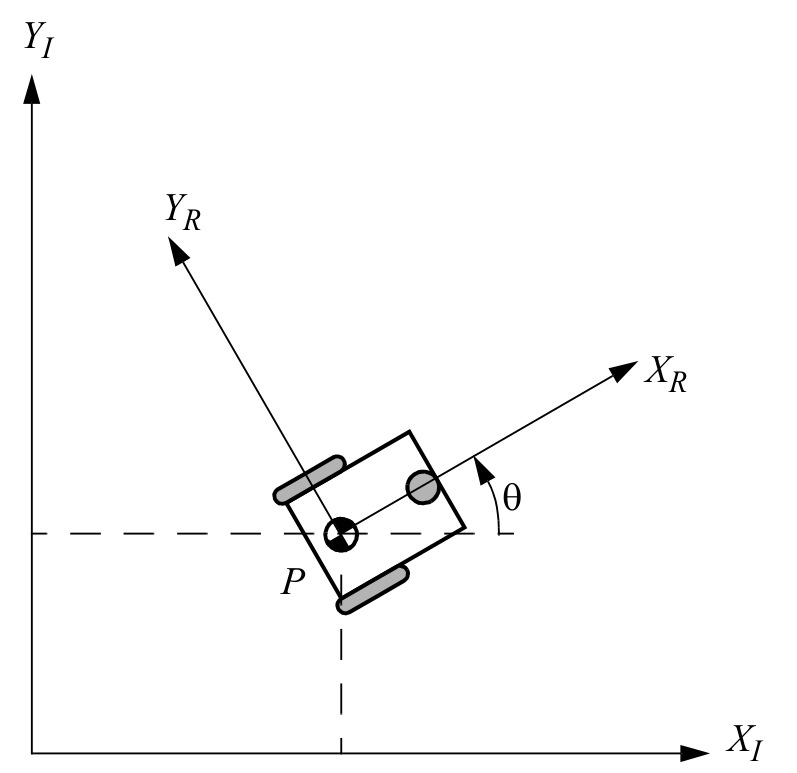
\includegraphics[width=0.4\linewidth]{fk}
    \caption[Forward kinematics of mobile robot.]{Forward kinematics of mobile robot \cite{siegwart2011introduction}.}
    \label{fig:fk}
\end{figure}

Considering the robot from \prettyref{fig:fk}, the position according to the global coordinate system can be represented by $\xi_I = [x, y, \theta]$ and the velocity $\dot{\xi} = [\dot{x}, \dot{y}, \dot{\theta}]$. The velocity model for the robot coordinate system can be written as \cite{siegwart2011introduction}:

\begin{equation}
\dot{\xi_R} = 
\begin{bmatrix}
\cos \theta && \sin \theta && 0 \\
- \sin \theta  && \cos \theta && 0 \\
0 && 0 && 1
\end{bmatrix}
\cdot 
\begin{bmatrix}
\dot{x} \\
\dot{y} \\
\dot{\theta}
\end{bmatrix}
=
R(\theta) \cdot \dot{\xi_I}
\end{equation}

It is easy to calculate the inverse problem using the inverse matrix $R^{-1}(\theta)$, converting back from the robot coordinate frame to the global frame. The only missing parameter is how the wheel kinematics translates to the $\dot{\xi_R}$ robot velocity, and that will depend on the robot wheel arrangement (wheel type, number of wheels, radius) and the robot dimensions.

The main disadvantages of wheel odometry are that the robot is limited to flat terrain, and even then slippery and small changes to forward kinematics (i.e. the radius of the wheel changes slightly) can accumulate error over time, as there is not a suitable way to correct the error without other sources of information.

\subsection{Laser odometry}

Laser odometry bases itself on Laser Scanner data to localize the robot. Instead of using odometry to watch how the robot moves in the environment, it uses the collected data to see how the environment moves in relation to the robot.

One approach to this calculation would be taking two consecutive laser scanners and comparing them. It is assumed that the environment is mostly static so not much should change from one set of data to the other. The transformation that minimizes the distance between points from the two sets is then considered to be the movement of the robot in that time slot \cite{Jaimez_et_al_ICRA2016}.

As the small movements are integrated over time, this approach has the same flaws as wheel odometry, with error accumulating over time. However, the robot can improve accuracy by keeping a laser scanner measurement history and repeating the minimization between many poses. It can also take advantage if it revisits a point in the past where the measurement was more accurate, as it can use data from that measurement for comparison.

\section{The localization and mapping problem}

The localization process can be expressed mathematically as follows \cite{thrun2005probabilistic}. Since all the measurements are discrete and supposing we want the localization of the robot through time, the set of poses over time can be represented as:

\begin{equation}\label{eq:x}
    X_t = \{x_0, x_1, \dots, x_t\} 
\end{equation}

The map can also be represented by a variable $M$ as follows. Notice also that the map is considered to be time-invariant in this case, and only depends on $n$ which is the number of features in the world.

\begin{equation}
    M = \{m_0, m_1, \dots, m_{n - 1}\}
\end{equation}

In order to evaluate both variables $X_t$ and $M$, it is necessary to have some idea on how the robot is interacting with the world. This can be for instance the measurements of robot odometry (wheel or laser odometry) or IMU data. The set of these measurements is defined as:

\begin{equation}
    U_t = \{u_0, u_1, \dots, u_t\}
\end{equation}

To also build the map, the robot will need the set of observations of the world, that can come as measurements from 3D cameras, LIDAR, sonar, etc. This set of measurements is defined as:

\begin{equation}
    Z_t = \{z_0, z_1, \dots z_t\}
\end{equation}

Since every measurement is noisy, the position can only be represented as a \textit{belief}, where the belief is the probability that the robot is in a position given the set of inputs and measurements. This belief depends on the set of observations from the past. This can be represented as:

\begin{equation}
    bel(x_t, M) = p(x_t, M | u_{1, t}, z_{1,t})
\end{equation}

There are three main approaches to solve this problem and calculate the belief: Extended Kalman Filters, Particle Filters, and Graph-based.

One of the concerns of mobile robots is how to build a map that is compatible with the environment and represents obstacles properly. While in some applications it is possible to have a pre-compiled map from the environment using the floor plan as a reference, those can be obsolete when dealing with highly dynamic environments or when objects get in the way. Even in static environments, there is a need to compensate for faulty or noise sensors, errors in the localization, and the pre-compiled maps should only be used as complementary information. One of the techniques that emerged to solve these problems, and later was adopted as the core of many SLAM algorithms, is the occupancy grid \cite{elfes1989using} representation.

The occupancy grid is a form of representing obstacles in 2D or 3D where each cell on the grid stores the probabilistic information of that area. This especially useful because it provides a comprehensive way to fuse sensor data, based on probability, instead of out-of-the-box algorithms that require fine tuning to work.

\begin{figure}[!ht]
    \centering
    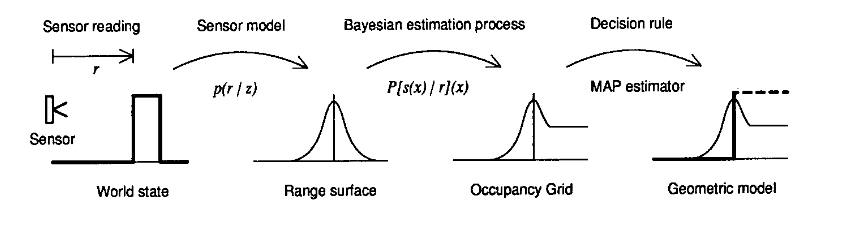
\includegraphics[width=.9\linewidth]{grid_steps}
    \caption[Steps when building an occupancy grid.]{Steps when building an occupancy grid \cite{elfes1989using}.}
    \label{fig:grid_steps}
\end{figure}

According to \prettyref{fig:grid_steps}, the first step when building a sensor grid is to get the sensor reading. The next step is build a sensor model $p(r|z)$. Then, the Bayesian estimation is applied, based on all the observations before and current observations, to update the map. Finally, the world model is obtained using an estimator such as \textit{maximum a posteriori} (MAP). All those steps are done by the SLAM algorithms using different techniques. Even with default tuning, those algorithms are good enough to work on most scenarios.

Naturally, the obstacle cell is labeled as occupied, with probability 1. All the cells until this one are labeled as empty, with probability 0. The unknown cells are labeled unknown, with probability 0.5. \prettyref{fig:occupancy_grid} show the graphical representation of this process.

\begin{figure}[!ht]
    \centering
    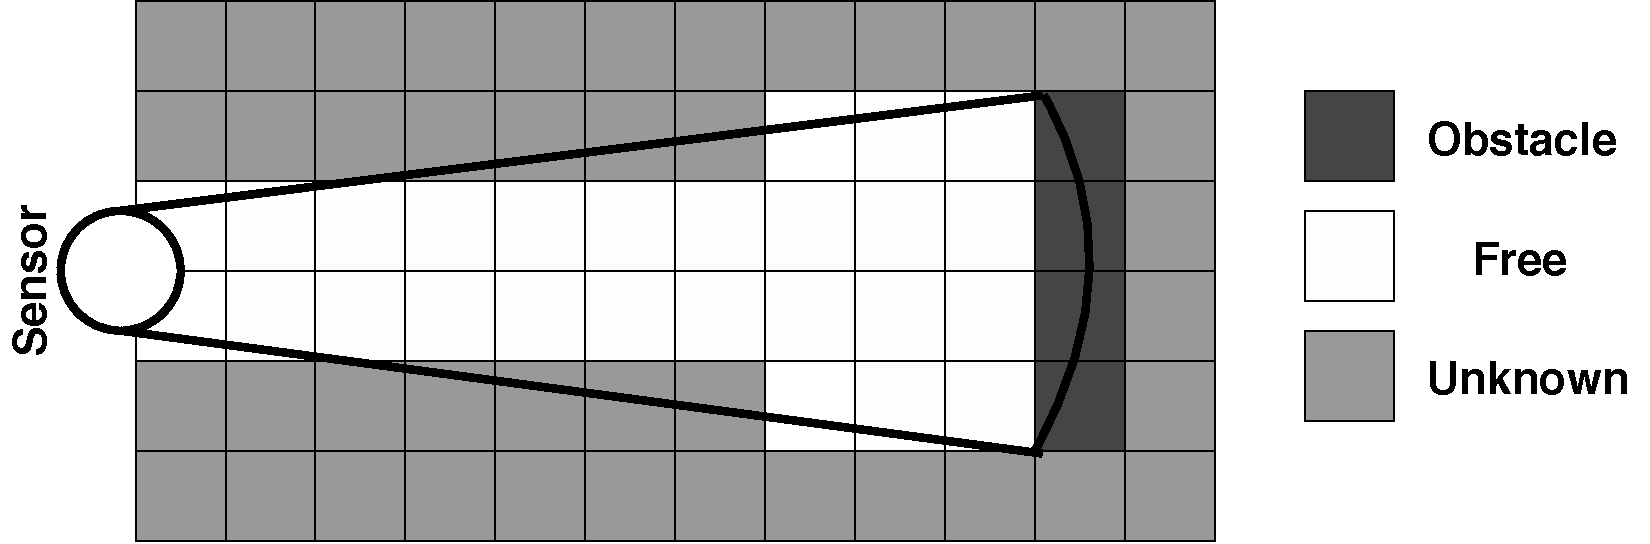
\includegraphics[width=.9\linewidth]{occupancy_grid}
    \caption{Illustration of occupancy grid for a single sensor.}
    \label{fig:occupancy_grid}
\end{figure}

The process is iterative and, as measurements from different points of view and different sensors grow, the maps become more and more complete, as shown on the occupancy grid proposed by \citeauthor{elfes1989using} seen on  \prettyref{fig:occupancy_grid_algorithm}. Data fusion between sensors can also be done to build a more accurate global map.

\begin{figure}[!ht]
    \centering
    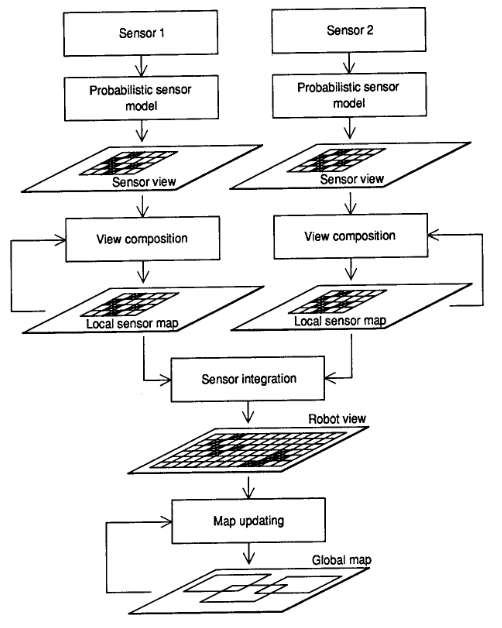
\includegraphics[width=.9\linewidth]{occupancy_grid_algorithm}
    \caption[Occupancy grid algorithm for multiple sensors proposed by Elfes.]{Occupancy grid algorithm for multiple sensors proposed by \citeauthor{elfes1989using}.}
    \label{fig:occupancy_grid_algorithm}
\end{figure}

\section{ROS SLAM algorithms}

\subsection{Gmapping}

Gmapping is by far the most famous SLAM algorithm in robotics for a number of reasons. It was originally proposed by \citeauthor{doucet2000rao} in 2000 as a way of combining particle filter algorithms with Rao-Blackwellized techniques. The main advantage of their approach is dealing with non-gaussian distributions that Kalman filters cannot deal with without rough linearization, as well as being less complex to implement.

In \cite{grisetti2007improved}, Grisetti proposed improvements to \citeauthor{doucet2000rao} techniques in order to reduce complexity and make the resampling step better. It works by first reducing the number of particles needed to be stored combining the current laser scan observation and odometry information, contrary to previous approaches where only odometry was used, reducing the estimation error and getting a more refined map. The second technique is using adaptative resampling, meaning that resampling only has to be done when needed, reducing the problem with particle depletion, when only a few particles are in high-probability areas and a lot of particles represent pretty old and unreliable information.

\subsection{Hector}

Hector SLAM first emerged in 2013 to solve the very specific problem of mapping in uneven terrains. It was aimed to be used in rescue robots that have to be robust enough to drive through ramps and obstacles and still be able to estimate the trajectory and map without reliable odometry information. Instead of trying to filter data to only include useful data, Hector pose estimation completely drops odometry data in favor of laser scanner data. It instead uses a fast LIDAR data scan-matching to estimate odometry. In order to estimate 6DOF when moving in uneven terrain, the algorithm also needs an IMU device, and optional localization devices like GPS, barometers, and accelerometers. All the data is then fused using an Extended Kalman Filter (EKF), and not including odometry information is a simple way to exclude all errors caused by wheel spin, drift or slippery ground \cite{kohlbrecher2011flexible}.

\subsection{Karto}

Karto is a graph-based SLAM algorithm developed by Karto Robotics and made open-source in 2010. Graph-based SLAM, proposed initially by \citeauthor{lu1997globally}, works by organizing the robot pose information into a graph and then optimizing it to make it more consistent and minimize an error function. While the construction of the graph is heavily sensor dependent, optimizing the graph is computationally expensive and the reason why Graph-based SLAM took so long to become popular \cite{grisetti2010tutorial}.

The graph is constructed representing every pose for the robot as a node in the graph. Every robot movement is then represented as an edge in the graph that connects the poses, this data in the edge usually being the odometry information. If the robot comes back to a known position, the algorithm does the loop closure and connects the graph to a previously known node. Since odometry is not reliable, it is corrected using the laser scanner measurements. The scan observation in both poses is then matched to calculate the virtual transformation that should map one measurement optimally to the other. Let $z_{i,j}$ be the odometry information between poses $i$ and $j$ and $\hat{z_{i,j}}$ be the expected measurement, the error $e_{i,j}$ can be calculated simply subtracting one from the other, i.e,

\begin{equation}
    e_{i,j}(x_i, x_j) = z_{i,j} - \hat{z_{i,j}}
\end{equation}

The goal is to ultimately build a function $F(x)$ using the log-likelihood strategy:

\begin{equation}
    F(x) = \sum_{\langle i, j \rangle \ \in \ \mathcal{C}} e_{i,j}^T \Omega_{i,j} e_{i,j}
\end{equation}

\noindent so that it can be minimized by the optimization algorithm for $x^*$, i.e, 

\begin{equation}
    x^* = \text{argmin}_x \ F(x) \,.
\end{equation}

In order words, the questions is what is the optimal path that minimizes the observed error, given the distribution $\Omega$ and the measurements $z$ and $\hat{z}$. The optimization is the main problem when dealing with graph-based SLAM, and many different approaches exist to solve this problem. Karto uses Sparse Pose Adjustment, which takes advantage of the sparsity on the large matrices required to solve the optimization problem \cite{konolige2010efficient}.

\subsection{Cartographer}

Cartographer is a fairly recent SLAM technique developed by Google. The concept behind the algorithm can be seen on \prettyref{fig:cartographer}. The main idea is separating SLAM into two different problems: local SLAM and Global SLAM. The main objective is not having to deal with big maps or representations while mapping a new area. Instead, a submap is created for the local area and updated every new scan. Every scan is also tested against the submap using a Ceres-based scan matcher, to do pose optimization.

The idea of having submaps is that it is only built using a few scans, meaning that the estimate should be very close to reality. As the submaps grow larger, so does the error, meaning that at every few scans a new submap is started. The Global SLAM thread will then have a collection of submaps to compute the whole map running loop closure \cite{cartographer2016google}.

\begin{figure}[!ht]
    \centering
    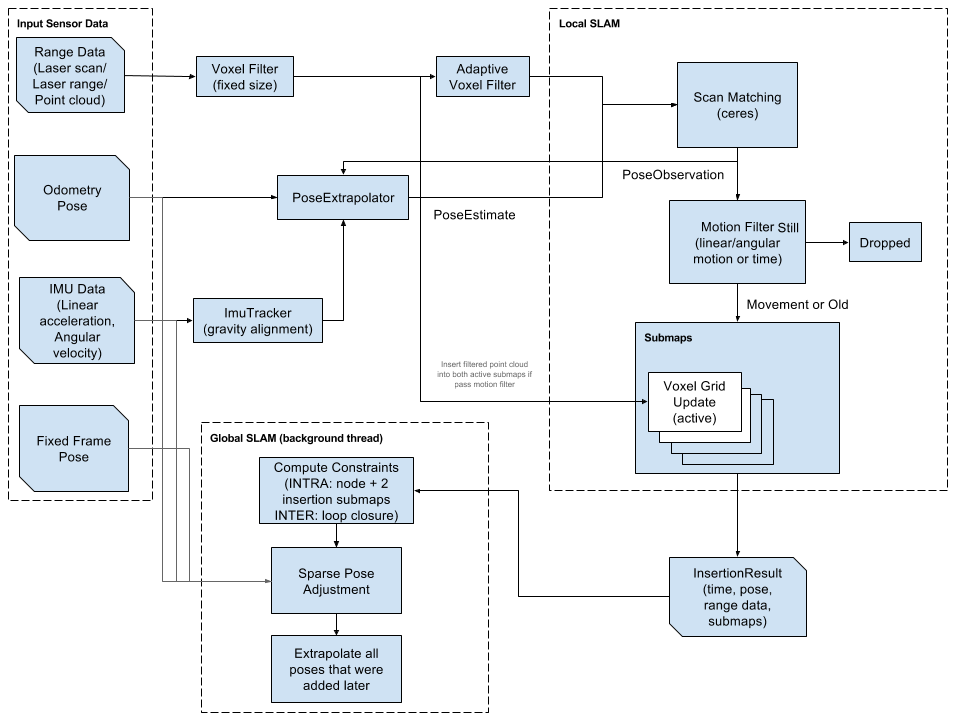
\includegraphics[width=\linewidth]{cartographer}
    \caption[High-level System overview of Cartographer.]{High-level System overview of Cartographer \cite{cartographerimage}.}
    \label{fig:cartographer}
\end{figure}

\section{Evaluating SLAM performance} \label{sec:evaluating}

There is a lot of debate on how to evaluate SLAM performance. Since there are plenty of algorithms using different techniques, each one of them having their own set of parameters, there is a need to evaluate them and tell which one does better in each scenario. A lot of this evaluation is done visually, assisted by a human that tells whether the occupancy grid is adequate considering the building floor plans. But as SLAM algorithms get more precise, it is difficult to draw conclusions just from the appearance itself. Additionally, there is the problem of not having the floor plants for publicly available datasets, making it harder to compare between methods \cite{kummerle2009measuring}.

According to \citeauthor{amigoni2007good}, the following issues have to be addressed when comparing SLAM:

\begin{itemize}
    \item The dataset must be publicly available, examples being MIT Killian Court or the Intel Research Lab dataset \cite{kummerle2009measuring}.
    \item All algorithm parameters have to be indicated.
    \item The behavior for the algorithm has to be tested with different parameters in order to evaluate robustness.
    \item The dataset must include a closed-loop test, where the robot runs around an environment and comes back to the same place, to test against algorithm divergence.
    \item The ground truth must be used to evaluate results when available.
    \item Bad mapping results must be shown.
\end{itemize}

The most natural way of analyzing the poses is the squared error from the pose estimates against the ground truth. By calculating the distance from one to another and adding over time, we can get a good metric for the pose error. Considering the $x_i$ as the pose calculated by the SLAM and $x_i^*$ the ground truth pose and $N$ the total number of poses, we can derive the squared error $\epsilon(x)$ as follows:

\begin{equation}\label{eq:error_squared}
\epsilon(x) = \frac{1}{N} \sum_{i = 1}^N (x_i - x_i^*)^2 \,.
\end{equation}

\citeauthor{kummerle2009measuring} proposes a framework to analyze mapping accuracy that uses visual inspection in order to estimate the relations between the robot poses and the environment. The estimation is then compared to the SLAM results and the final metric is the "deformation energy" required to transform the mapped result into ground truth. In other words, each of the $N_c$ displacements $\delta_{i,j}$ is compared against the ground truth $\delta_{i,j}^*$ using $\epsilon(\delta)$ given by

\begin{equation}\label{eq:displacement}
    \epsilon(\delta) = \frac{1}{N_c} \sum_{i, j} trans(\delta_{i,j} \ominus \delta_{i,j}^*)^2 + rot(\delta_{i,j} \ominus \delta_{i,j}^*)^2
\end{equation}

 \noindent for a set of  $(i,j)$ pairs. The displacement $\delta_{i, j}$ is simply calculated by the transformation from a local measurement between two known poses, from pose $x_i$ to pose $x_j$, using a distance function like the Euclidian Distance. Evaluating the displacement instead of the global position is great because it makes the evaluation resilient to small errors at the start of mapping that would impact every subsequent global position, even when the mapping in the next steps is done correctly. Since the ground-truth displacement is not available, this implementation relies on the fact that the relation between two poses can be calculated using the laser scanner, each pose later evaluated by a human. It also relies on a good enough initial guess, also human assisted. The authors also assume just evaluating the poses without evaluating the resulting map is enough for SLAM benchmarking. While this holds true for most cases, it is still very hard to infer global performance, as global displacements (large enough distance between $i$ and $j$) also carry the problem of accumulating human error, as each measurement is supervised.
 
 \citeauthor{santos2013evaluation} propose a more in-depth comparison with the publicly available SLAM algorithms that run on ROS. The authors ran both noise-free simulation and real-life experiments with the scenarios and analyzed. The maps collected were binarized and aligned and error metric was defined as the normalized sum of distances from all pixels in the resulting map to its nearest neighbour in the ground-truth map. The error metrics were analyzed, also evaluating the CPU usage for each algorithm. The authors, however, didn't provide extensive information on how the maps were aligned, very crucial since the fit has to be optimal in order to do an adequate comparison.
 
 \section{Proposed evaluation techniques} \label{sec:proposed-evaluation}
 
 In order to better evaluate the algorithms, general guidelines will be respected:
 
 \begin{itemize}
     \item Algorithms available in ROS will be used, to ensure every algorithm is publicly available for testing.
     \item Different maps will be tested to ensure no algorithm is favored. In each run, each algorithm will receive the same working data in the form as ROS bags.
     \item The scenario will be simulated in a map carefully generated using a public tool, to make sure everyone can generate the same testing data.
     \item Maps will test the ability for the algorithm to do accurate mapping, accurate localization, and loop-closure. Different metrics will be used to ensure all these three aspects of each map are analyzed.
     \item Each algorithm will be run using their default configuration. The goal is to test how each algorithm performs in the general case, instead of finding the optimal configuration that gives us the best results for a specific test.
 \end{itemize}
 
The manuscripts discussed in \prettyref{sec:evaluating} already give us a good indication of what to aim for in a comparison algorithm. The first metric chosen is the one described in \cite{kummerle2009measuring}, as it best describes local error in the form of displacements when analyzing the trajectory of the robot. Since the ground-truth data is now available and doesn't have to be inferred by a human operator, the process can be done autonomously and we can ensure the data perfectly matches the environment. For comparison, we are also going to include the squared error metrics proposed in \prettyref{eq:error_squared}.

The second comparison method chosen is the one demonstrated in \cite{santos2013evaluation}, only that now the approach for lining up the maps and calculating the error metric will be fully described. This approach will help to analyze the quality of the generated map regarding the placement of walls and objects, including their orientation and the amount of noise.

The third metric will focus on analyzing the modeled empty space of each algorithm, to see if the area of the generated room matches the area of the map. This is useful in combination with the last algorithm to see how good is the scale on each map.

\section{Experimental maps}\label{sec:selecting_maps}

The maps have to be designed to include the scenarios encountered in real life. Three maps were designed and can be seen in \prettyref{fig:generated_maps}. The selection aims at testing three key elements in SLAM: loop closure, scale and localization.

\begin{figure}[!ht]
     \centering
     \subfloat[][]{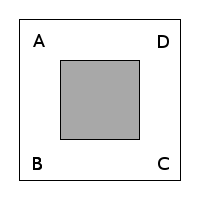
\includegraphics[width=.3\linewidth]{test1_coordinates}\label{subfig:test1}}
     \subfloat[][]{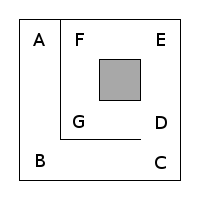
\includegraphics[width=.3\linewidth]{test2_coordinates}\label{subfig:test2}}
     \subfloat[][]{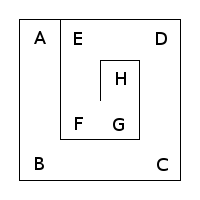
\includegraphics[width=.3\linewidth]{test3_coordinates}\label{subfig:test3}}
     \caption{Selected maps for testing.}
     \label{fig:generated_maps}
\end{figure}

The first map can be seen on \figurename~\ref{subfig:test1}. It is meant to test the loop closure capabilities of each algorithm since the robot will have to do the full circle, come back to the same point, and then connect the two pathways. The robot starts at the A position, goes into a straight line into B, then into a straight line into C. It then spins once around itself, goes to D and finally comes back to A.

The second map seen on \figurename~\ref{subfig:test2}. It is a more complex version of the first map. It will test the capability of the algorithm to maintain scale between different rooms, as the corridor on the left and the loop on the right are separated by walls. The robots starts at A and follows the sequence ABCDEFG. It then returns to the home position through D, totalling ABCDEFGDCBA.

The third map, shown on \figurename~\ref{subfig:test3}, will test how the localization performs without revisiting positions, as the robot goes to the center of the loop without previous information and then comes back. The sequence followed is ABCDEFGHGFEDCBA.

\section{Pose metrics} \label{sec:metrics}

\prettyref{sec:proposed-evaluation} presented the metrics that will be used to evaluate the algorithms. \prettyref{fig:metrics} illustrates some of the measurements that are taken between two estimated poses $x_i$ and $x_j$, in green, and two ground-truth poses, $x_i^*$ and $x_j^*$, in red.

\begin{figure}[!ht]
    \centering
    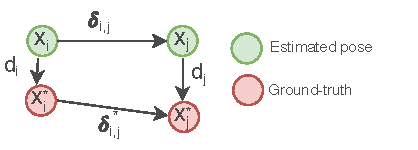
\includegraphics[width=.9\linewidth]{metrics}
    \caption{Representation of metrics taken.}
    \label{fig:metrics}
\end{figure}

Recalling \prettyref{sec:localizing}, the robot position relative to the global reference frame can be represented by two coordinates for the Cartesian position and one for the orientation. Let's define $x_i = [x^c_i, y^c_i, \theta_i]$ and $x_j = [x^c_j, y^c_j, \theta_j]$.

The displacements $\delta_{i,j}$ and $\delta_{i,j}^*$ are calculated by taking the relative transformation between two poses $i$ and $j$:

\begin{equation}
\delta_{i,j} = x_j - x_i =
\begin{bmatrix}
x^c_j - x^c_i \\
y^c_j - y^c_i \\
\theta_j - \theta_i
\end{bmatrix} \,.
\end{equation}

The goal is to calculate the contributions $trans(\delta_{i,j} \ominus \delta_{i,j}^*)$ and $rot(\delta_{i,j} \ominus \delta_{i,j}^*)$, respectively the linear displacement and the angular displacement. As mentioned, these transformations can be calculated using the Euclidian distance as following:

\begin{equation}
trans(\delta_{i,j} \ominus \delta_{i,j}^*)^2 =
((x^c_j - x^c_i) - (x^{c*}_j - x^{c*}_i))^2 + 
((y^c_j - y^c_i) - (y^{c*}_j - y^{c*}_i))^2 \,,
\end{equation}

\begin{equation}
rot(\delta_{i,j} \ominus \delta_{i,j}^*)^2 = 
((\theta_j - \theta_i) - (\theta_j^* - \theta_i^*))^2 \,.
\end{equation}

\citeauthor{kummerle2009measuring} proposes to select the pairs $(i,j)$ from the dataset using scan matching evaluated by a human operator. Since our dataset have the ground-truth, all possible displacements can be evaluated. Given a set o $N$ poses, the linear displacement can then be represented by:

\begin{equation}
\text{Linear displacement} = \frac{1}{N^2} \sum_{i = 1}^N \sum_{j = 1}^N trans(\delta_{i,j} \ominus \delta_{i,j}^*)^2
\end{equation}

\noindent and the angular displacement by:

\begin{equation}
\text{Angular displacement} = \frac{1}{N^2} \sum_{i = 1}^N \sum_{j = 1}^N rot(\delta_{i,j} \ominus \delta_{i,j}^*)^2
\end{equation}

The squared error is easier to calculate, as it relates only to the current pose. We can define the same separate metrics for the translation and rotation from the estimated pose to the ground-truth pose:

\begin{equation}
trans(d_i)^2 = (x^{c*}_i - x^{c*}_i)^2 + (y^{c*}_j - y^{c*}_j)^2
\end{equation}

\begin{equation}
rot(d_i)^2 = (\theta_i - \theta^*_i)^2 \,.
\end{equation}

The individual pose errors are then summed across the trajectory and normalized according to the following equations:

\begin{equation}
\text{Linear squared error} = \sum_{i=1}^N \frac{1}{N} trans(d_i)^2 \,,
\end{equation}

\begin{equation}
\text{Angular squared error} = \sum_{i=1}^N \frac{1}{N} rot(d_i)^2 \,.
\end{equation}

\section{Map alignment metric} \label{sec:icp}

Once the map is saved, we have both the reference map and the generated map, as shown in \prettyref{fig:reference_map_icp}. We can then run an algorithm to align the maps properly, as suggested by \citeauthor{santos2013evaluation}.

\begin{figure}[!ht]
     \centering
     \subfloat[][Ground truth]{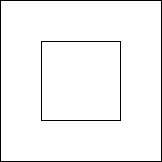
\includegraphics[width=.3\linewidth]{test1_cropped}\label{subfig:test1_cropped}}
     \hspace{2cm}
     \subfloat[][SLAM generated map]{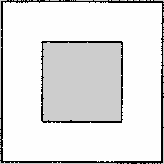
\includegraphics[width=.3\linewidth]{gmapping_test1}\label{subfig:test1_gmapping}}
     \caption{Occupancy grid representation of ground truth and SLAM generated map.}
     \label{fig:reference_map_icp}
\end{figure}

First, both maps are imported as a point cloud, each pixel representing a point in space, as shown in \prettyref{fig:point_cloud}. As you can probably tell, the image is twisted 90 degrees counter-clockwise when being read by the algorithm. This happens because the coordinate system for images is not the same as the Cartesian coordinate system.

\begin{figure}[!ht]
     \centering
     \subfloat[][Ground truth]{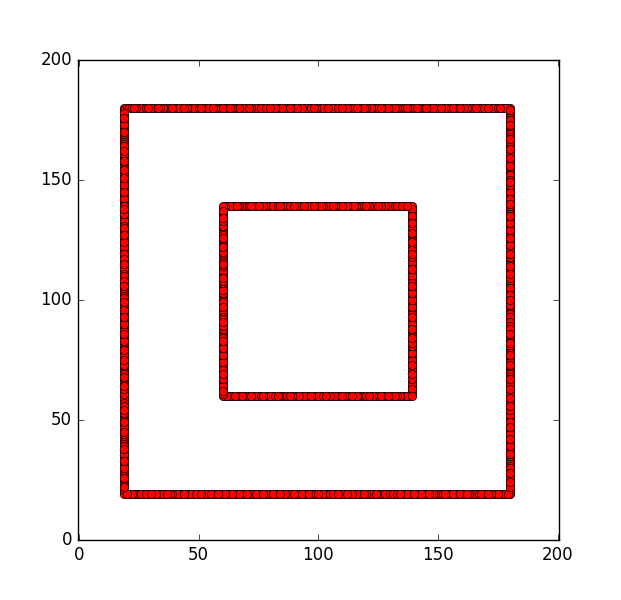
\includegraphics[width=.45\linewidth]{original_pcl}\label{subfig:original_pcl}}
     \hspace{0cm}
     \subfloat[][SLAM generated map]{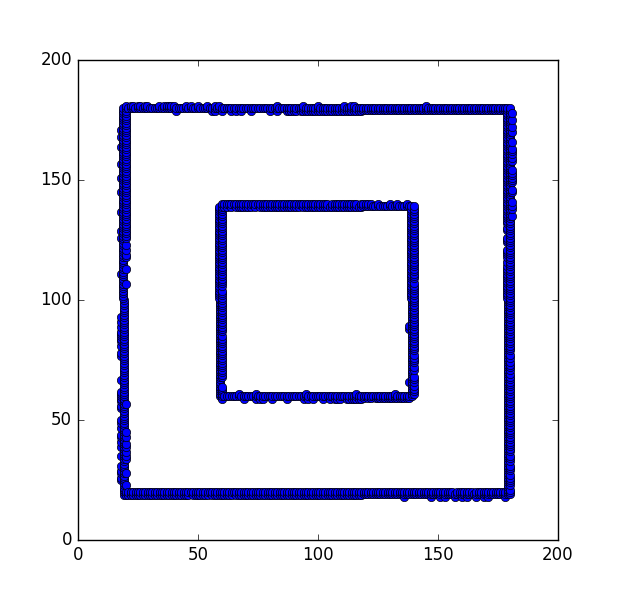
\includegraphics[width=.45\linewidth]{map_pcl}\label{subfig:map_pcl}}
     \caption{Point cloud representation of ground truth and SLAM generated map.}
     \label{fig:point_cloud}
\end{figure}

ICP, or Iterative Closest Point, is a state-of-the-art way of aligning 3D meshes. It works by finding the transformation that best aligns two distinct point clouds minimizing the error distance between them. For more information about ICP, refer to \citeauthor{besl1992method}.

The ICP algorithm used is the one provided by \citeauthor{flannigan2019}. It will calculate the transformation that best aligns the two maps shown in \prettyref{fig:point_cloud}. The aligned point cloud can be seen on \prettyref{fig:alignment_pcl}. To do that, we simply call the node launcher with the desired map and algorithm. 

\begin{figure}[!ht]
    \centering
    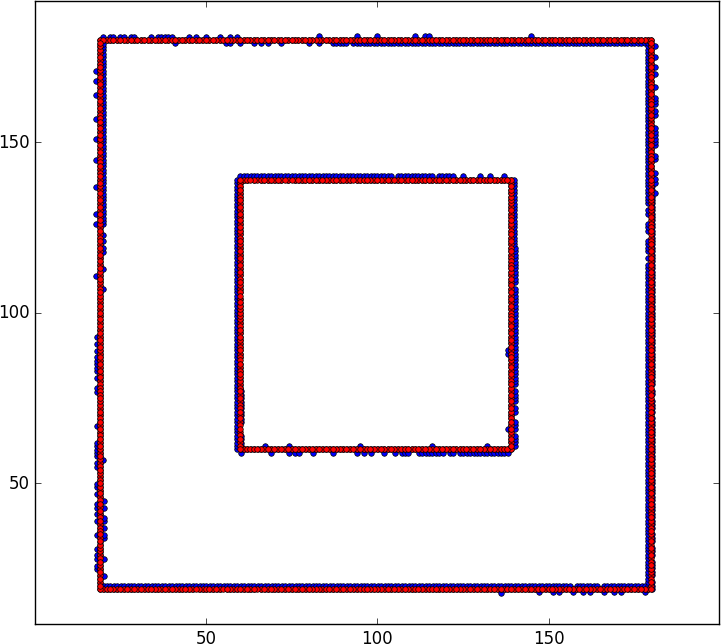
\includegraphics[width=0.45\linewidth]{alignment_pcl}
    \caption{Alignment of point clouds from \prettyref{fig:point_cloud}.}
    \label{fig:alignment_pcl}
\end{figure}

With the maps aligned, we then use the following equation

\begin{equation}
\epsilon(\text{map}) = \frac{1}{P} \sum_{i=1}^P dist(p_i - p_i^*(p_i))^2
\end{equation}

\noindent to calculate the error metric, where P is the number of points in \figurename~\ref{subfig:map_pcl}, $p_i$ represents one point in the data set and $p_i^*$ is the nearest neighbour of $p_i$ in the dataset shown on \figurename~\ref{subfig:original_pcl}. All the measurements are in pixels.

\section{Free space metric} \label{sec:free_space}

As important as placing the walls in the correct spots, metric that will be checked using ICP, is modeling free space correctly, where the robot can move. This is done by each algorithm by setting the pixels that are free as white. Those white pixels can be counted and checked against the free space in the original map. Since we only want a measurement of scale, we can use the following formula, where $w_o$ is the number of white pixels in the original image and $w_m$ is the number of pixels in the map generated by SLAM:

\begin{equation}
\epsilon(\text{space}) = \frac{w_o - w_m}{w_o} \times 100 \,.
\end{equation}

The signal of the result will also give indications about the mapping. If it is positive, it means that the original map has more white pixels than the mapped result, meaning the SLAM was more conservative and mapped less space than available. If it's negative, the algorithm actually mapped space that is not there, meaning the navigation layer will, later on, have to deal with this problem.